\documentclass{sig-alternate}
\usepackage[section]{algorithm}
%\usepackage[]{algorithm2e}
\usepackage{algorithmic}
\usepackage{balance}
\usepackage{makecell}
\usepackage[usenames,dvipsnames]{color}
\usepackage[10pt]{moresize}
\usepackage[font=small,skip=0pt]{caption}
\usepackage{dblfloatfix}

\setlength{\abovecaptionskip}{10pt plus 0pt minus 2pt}
%\newenvironment{definition}{\begin{defn}\begin{em}}{\end{em}\end{defn}}
\newcommand{\inred}[1]{{\color{BrickRed}\sf\textbf{\textsc{#1}}}}
\newcommand{\card}[1]{|#1|}
\newcommand{\norm}[1]{\left\lVert#1\right\rVert}
\newcommand{\bfd}{\mathbf{d}}
\newcommand{\bfu}{\mathbf{u}}
\newcommand{\bfq}{\mathbf{q}}
\newcommand{\Z}{\mathbb{Z}}
\DeclareMathOperator*{\argmin}{arg\,min}
\DeclareMathOperator*{\argmax}{arg\,max}
\newtheorem{definition}{Definition}
\newtheorem{theorem}{Theorem}[section]
\newtheorem{thm}{Theorem}[section]
\newtheorem{lemma}[theorem]{Lemma}
\newtheorem{proposition}[theorem]{Proposition}
\newtheorem{corollary}[theorem]{Corollary}
\newtheorem{Assumption}[theorem]{Assumption}
\newtheorem{Condition}[theorem]{Condition}
\newtheorem{exe}
[thm]{Exercise}
\newtheorem{eg}[thm]{Example}
\newtheorem{conj}[thm]{Conjecture}
\newcommand{\comment}[1]{\frameit{Comment}{#1}}%
\newcommand{\note}[1]{\frameit{Note}{#1}}
\newcommand{\todo}[1]{\frameit{To-do}{#1}}
\newcommand{\inote}[1]{\inred{$<<<${#1}$>>>$}}
\newcommand{\frameit}[2]{
    \begin{center}
    {\color{BrickRed}
    \framebox[3.3in][l]{
        \begin{minipage}{3in}
        \inred{#1}: {\sf\color{Black}#2}
        \end{minipage}
    }\\
    }
    \end{center}
}

\usepackage{etoolbox}
\makeatletter
\patchcmd{\maketitle}{\@copyrightspace}{}{}{}
\makeatother


\begin{document}

\sloppy
\newcommand{\para}[1]{\par \bigskip \noindent {\bf #1.}}
\newcommand{\spara}[1]{\par \bigskip \noindent {\sc #1.}}

\newcommand{\ymatrix}[1]{\mathbf{#1}}
\newcommand{\yvector}[1]{\mathbf{#1}}
\newcommand{\ytrans}[1]{#1^{\mathsf{T}}}

\newcommand{\yset}[1]{\mathcal{#1}}
\long\def\/*#1*/{}
%

\title{Click-Based Content Recommendation for Hierarchical Semantic Streams}
%\subtitle{[Extended Abstract]
%\titlenote{A full version of this paper is available as
%\textit{Author's Guide to Preparing ACM SIG Proceedings Using
%\LaTeX$2_\epsilon$\ and BibTeX} at
%\texttt{www.acm.org/eaddress.htm}}}
%
% You need the command \numberofauthors to handle the "boxing"
% and alignment of the authors under the title, and to add
% a section for authors number 4 through n.
%
% Up to the first three authors are aligned under the title;
% use the \alignauthor commands below to handle those names
% and affiliations. Add names, affiliations, addresses for
% additional authors as the argument to \additionalauthors;
% these will be set for you without further effort on your
% part as the last section in the body of your article BEFORE
% References or any Appendices.

\numberofauthors{6}
%\author{
%\alignauthor Youssef Billawal \\
%\email{\normalsize billawal@yahoo-inc.com}\\
%\alignauthor Karolina Buchner \\
%\email{\normalsize karolina@yahoo-inc.com}\\
%\alignauthor Yunjiang Jiang \\
%\email{\normalsize jyj@yahoo-inc.com}\\
%\alignauthor Tina Liu\\
%\email{\normalsize tliu@yahoo-inc.com}\\
%\alignauthor Rao Shen\\
%\email{\normalsize raoshen@yahoo-inc.com}\\
%\alignauthor Ruiqiang Zhang\\
%\email{\normalsize ruiqiang@yahoo-inc.com}\\
%}

\author{
Yunjiang Jiang\\
\email{\normalsize jyj@yahoo-inc.com}\\
\and
Ruiqiang Zhang\\
\email{\normalsize ruiqiang@yahoo-inc.com}\\
\and
Rao Shen\\
\email{\normalsize raoshen@yahoo-inc.com}\\
\and
Karolina Buchner\\
\email{\normalsize karolina@yahoo-inc.com}\\
\and
Tina Liu\\
\email{\normalsize tliu@yahoo-inc.com}\\
\and
Sudharshan Lamkhede\\
\email{\normalsize lamkhede@yahoo-inc.com}\\
\and
Youssef Billawala\\
\email{\normalsize billawal@yahoo-inc.com}\\
}
\maketitle
\begin{abstract}

We design a unified recommendation system for hierarchical personalized news 
streams, using three sequential phases to optimize for serving-time 
efficiency. Within each phase we use user click count feedbacks as training 
signals. This solves the issue of insufficient training labels in the context 
of content multi-classification (phase 0). In the personalization stage, we 
judiciously balance multilinear regression (phase 1) with gradient boosting 
models (phase 2) to ensure coverage, recency, and relevance at the same time, 
while maintaining low latency. The models include various features inspired by 
recency, personalization, popularity, and target stream. Significant 
improvements are observed in both offline experiments and online bucket test. 

\end{abstract}

% A category with only the three required fields
\category{H.3.m}{Information Search and Retrieval}{Miscellaneous}

\terms{Algorithms, Information Retrieval}

\keywords{News  recommendation, Information retrieval, Personalization, Semantic stream classifier, Multi-stream recommendation, Recency}


\section{Introduction}



Developing efficient and accurate personalized recommendation systems of 
news-worthy content has been a focus of today's media industry. 
On the one hand search engines have enabled users to locate articles or 
multimedia content of any topic within a few keystrokes. On the other hand, 
users are constantly overwhelmed by the amount of information generated 
daily, much of which is irrelevant to their personal interest. Thus 
directory-style news streams organized by topics are becoming increasingly 
popular. 

Under the latter framework, we not only need to recommend generically interesting articles, but those within a specific category, such as sports, finance, or technology, to a diverse array of users. Underneath each broad category lies more sub-categories that facilitate users to find relevant and interesting content quickly (Figure~\ref{hierarchy}).
\begin{figure*}
\centering
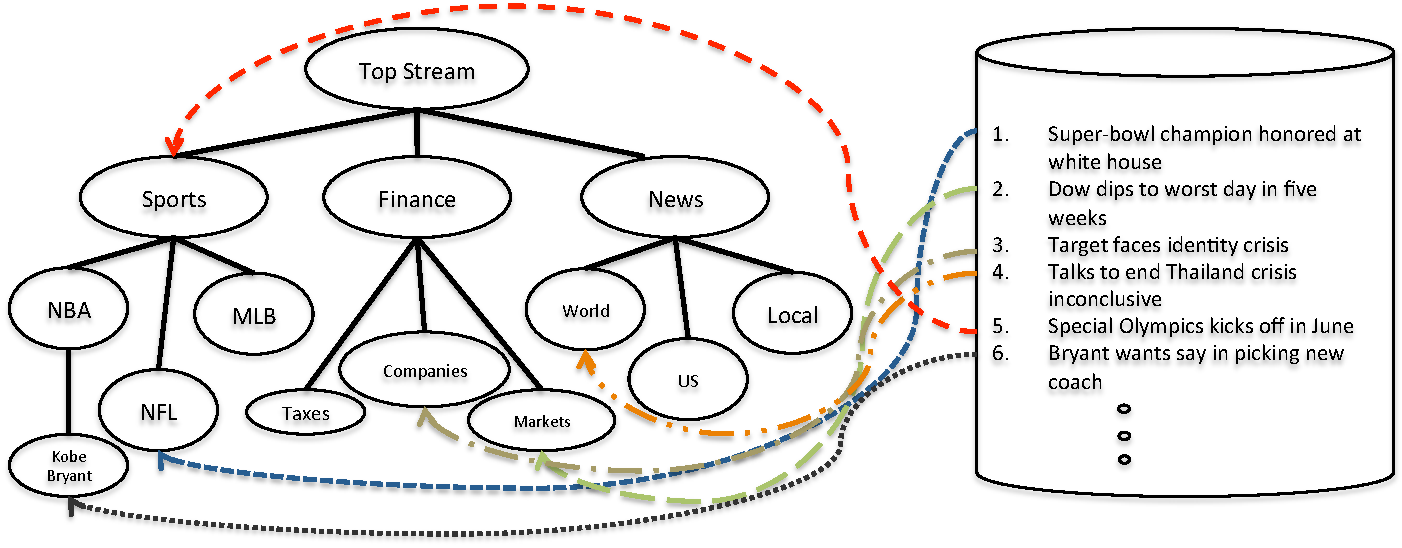
\includegraphics[scale=0.5]{Hierarchy.pdf}
\caption{Semantic Stream Hierarchy} \label{hierarchy}
\end{figure*}

Different from traditional news recommendation for a single stream, the first 
challenge is to assign articles into corresponding semantic streams as shown 
in the figure. One obvious approach is to implement a document filter for each 
category node on the content hierarchy.  However, the semantic streams are not 
static structures. It is evolving. To train a new document filter requires the 
labeling of training 
examples. Given the number of streams (easily in the 1000's) in question and 
its dynamic property, it is impossible to solve it by editorial resource.
But document filter is still useful as a starting point. We address the 
problem with a combination of user click feedbacks and editorial labeling 
(phase 0).


To solve the ranking problem under stringent runtime constraints, we propose a 
system design with 2 components: a coarse linear ranking step followed by a 
fine gbdt based step. 
Altogether, the three phases yield an efficient approximate solution to the optimal ranking problem; an exact solution is clearly too expensive for any reasonably sized content/user pools.

The paper is organized as follows. Stream classifier is described in 
section~\ref{sec:system design} including feature source discussion 
(\ref{sec:feature engineering}, stream classifier(section~\ref{sec:stream 
classifier}), Phase 1 ranking (~\ref{sec:phase1 ranking}) and Phase 2 ranking 
(~\ref{sec:phase2}). Experimental results are in section~\ref{sec:experiments} 
where we describes metrics, phase 0, phase 1 and phase 2 results. 
Section~\ref{sec:conclusions} concludes the paper.



\section{Related Work}
\input related

\section{System Design}
\label{sec:system design}

\subsection{Motivations}
Designing an actionable system for thousands of article streams with millions 
of contents to present is a highly nontrivial task that requires both latency 
consideration and machine learning insight. The latter can further be divided 
into several categories of objectives, such as relevance, freshness, 
personalization, segmented popularity, etc. In order to build an agile and 
well-focused pipeline, it is imperative to modularize the effort into 
different phases. Thus we devote a document classifier phase (phase 0) to 
optimize for relevance, a pre-screening stream-specific linear matching phase 
(phase 1) to optimize for serving-time latency, followed by a more powerful 
ranking algorithm (phase 2); both phase 1 and phase 2 take into account 
personalization and popularity.  In general, having a multi-phase system can 
be a challenge in bucket tests or even offline optimization. Fortunately, due 
to their conceptual independence, we argue that it is relatively harmless to 
optimize them in parallel. 


\subsection{Phase 0: Stream Classifier}
\label{sec:stream classifier}

In the past the classification task for semantic streams was trivialized to 
the manual selection of logical filter criteria based on a basket of 
pre-engineered in-house features such as wikis and ycts aboutness scores. One 
could argue that not 
all classification criteria can be compactly summarized by a handful 
(certainly fewer than 100) of logical conjunctives and disjunctives. 
As we 
will show in the experimental results section below, even with simple 
unigram model, the precision-recall of a freshly trained model well 
outperforms the ones based on logical filters constructed by domain experts. 
Even for a stream as clearly defined as NFL, brute force human filter 
construction reveals that there are many edge cases, which lead to hundreds of 
terminal decision nodes. 

  As a baseline, we also consider the term-frequency 
  inverse-document-frequency (TFIDF) approach \cite{tfidf}, whereby a centroid 
  vector is constructed for each stream based on the number of appearances of 
  each token stem in the stream, weighted by the inverse of the logarithm of 
  the total number of documents in which it appears:
\begin{align*}
C^{\mathcal{S}}_{t_i} =\card{\{k \in [\dim \mathcal{S}]: \mathcal{S}_k = t_i  \}} / \log \card{\{d \in \mathcal{D}: t_i \in d\}}.
\end{align*}
Here $\mathcal{S}$ stands for the concatenated vector of all tokens from the training set articles in the stream, $C^{\mathcal{S}}$ stands for the centroid vector for the stream represented by $\mathcal{S}$, and $\mathcal{D}$ is the universal set of all documents.


\subsubsection{Data Collection}
  Independent of the model choice, it is important for us to choose a set of 
  positive and negative examples as our initial training set. Due to the large 
  quantity of articles and variety of topics in each stream, as well as the 
  sheer number of streams we are dealing with (ultimately in the thousands), 
  complete reliance on editorial judgment is infeasible. Instead we 
  opt for the following heuristic approach of labeling the articles as to 
  their appropriateness for a particular stream. 

  For the streams already in production, positive examples consist of articles 
  with clicks from at least 5 unique 
  users. The assumption is that users who visit a 
  particular stream are most likely interested in content pertaining to the 
  stream definition. Having multiple users interested in a document is a good 
  sign that the article is not just interesting from a general point of view, 
  but is also relevant to the stream. 
   
   Because of the low-recall concern with the above approach, we want to 
   avoid false negatives at the expense of true negatives. To ensure 
   scalability, we use the cold-start rule based filter to select negative 
   examples, but exclude the low click 
   count articles from training since they could be 
   unpopular due to either irrelevance or low quality.

  For streams not yet launched, domain expertise is required to 
  initialize the classifier. Fortunately we have a variety of well-polished 
  features, such as topical categories, tagged wiki entity, etc, that can be 
  combined through logical connectives to yield an approximate profile for the 
  stream. Once that gets launched and starts receiving user clicks, subsequent 
  batch active-learning cycles will be able to learn the model and fine-tune 
  it to suit the user interests. To avoid flooding a 
  specialized stream with generally popular topics, editorial judgments are 
  periodically injected as training samples. Other active 
  learning aspects of the model updating will be explored in future work.

\subsubsection{Feature and Model Selection}
We compared the relative performance of 4 distinct families of features: title 
and body token stems and frequency counts, yct and wiki aboutness score, 
editorial tags, and publisher ids.

While the topic 
category and publisher id together achieve high performance on testing, they 
perform poorly on editorial test. This is likely because we are merely 
relearning the rule based filter. On the other hand, token stem 
frequencies alone perform remarkably well on validation set compared to all 
other combination of features from the above list, so we choose them 
for all streams.

To determine the exact classifier form, we found that the performances 
of logistic loss and hinge loss (SVM) are comparable. Since our 
preferred training tool, Vowpal 
Wabbit~\footnote{https://github.com/JohnLangford/vowpal\_wabbit/wiki} with 
L-BFGS optimizer, supports logistic regression far better than SVM (as hinge 
loss is non-differentiable), we settled upon logistic regression. Some further 
exploration reveals that a ridge regularization parameter of $10$ works well 
for all three streams tested, and on both testing and validation sets. 

\subsection{Phase 1: Twisted Dot Product}
\label{sec:phase1 ranking}

The classifier instrumented at Phase 0 is not perfect, in particular we do not 
anticipate 100\% precision. Subsequent phases will remove any embarassing 
candidate article for each stream. The Stream Relevance Query (SRQ) proposed 
at Phase 1 can be viewed as an optimization step for the more serious ranking 
done at Phase 2. 

The production linear ranking uses the following formula:
\begin{align} \label{flat dotproduct}
\rm{score}_1 =  (\alpha_0  \rm{gmp} + \alpha_1  \langle \bfu,\bfd\rangle ) e^{-\beta \Delta T}.
\end{align}
Here $\bfu,\bfd$ denotes the user and dcument profile vectors respectively. 
$\rm{gmp}$ is a popularity score determined essentially by CTR of the article. 
$\Delta T$ is the time since publishing of the article, which captures the 
freshness of the article. Thus the exponential factor promotes more recent 
articles. The weights $\alpha_0, \alpha_1$, and $\beta$ are either trained 
offline or tuned with split online buckets. SRQ builds on \eqref{flat 
dotproduct} and takes the following form:
\begin{align} \label{original SRQ}
\rm{score}_{\rm{SRQ}} = (\alpha_0 \rm{gmp} + \alpha_1 \bfq_0 \cdot \bfd + \alpha_2 \bfq_1 \circ \bfu \cdot \bfd ) e^{-\beta \Delta T}.
\end{align}

$\bfq_0 $ and $\bfq_1$ are stream-specific feature vectors corresponding to 
document and user respectively. These are trained using real bucket user click 
data, before the other weights $\alpha_i$ are learned.  

The main issue is that the new stream-specific user 
profile $\bfu'$ can now have hundreds of thousands of nonzero entries, making 
it non-sparse and computationally intensive. So we instead consider the 
following practical SRQ model:

\begin{align} \label{practical SRQ}
\rm{score}_{\rm{pSRQ}} = (\alpha_0  \rm{gmp} + \alpha_1 \bfq \circ \bfu \cdot \bfd) e^{-\beta \Delta T}.
\end{align}
The main difference is the removal of the old-fashioned dot-product term. One could argue non-rigorously, that the Phase 0 filter is essentially performing the same job as the zeroth order term $\alpha_1 \bfq_0 \cdot \bfd$ in the original SRQ model. 

The output of Phase 1 ranking is a set of around 200 articles, to be ranked 
further by Phase 2 GBDT machinery. This reduction from thousands of articles 
facilitates highly sophisticated algorithms to be applied for accurate 
personalized ranking.

\subsection{Phase 2: Boosted Ranking}
\label{sec:phase2}
\input phase2


\section{Experiment Results}
\label{sec:experiments}

\subsection{Test Results}

\subsubsection{Phase 0}





The precision-recall curves for the three streams (Sports, Finance, and NFL) 
under linear classifier and tfidf approaches are shown in 
Figures~\ref{precision-recall}. The table~\ref{tab:precision} summarizes the 
training and test data used:
\begin{table}
\caption{Stream classifier training and test data}
\label{tab:precision}
\begin{tabular}{|l|l|l|}
\hline 
property & training size (+/-) & testing size (+/-) \\ \hline
Finance & 5410/33890 & 2287/14524\\ \hline
Sports & 6569/34947& 2821/14972\\ \hline
NFL & 1518/5054& 651/2167\\ \hline
\end{tabular}

\end{table}


Both training and test data are labeled according to the heuristic rule based 
on user clicks. For the linear classifier we use threshold at $0$, since the 
negative and positive examples are weighted equally. 


The table~\ref{tab:phase0exp} compares the point-wise precision-recall for 
smaller editorially labelled datasets, with the numbers of positive and 
negative examples chosen proportional to real world data. The third column 
shows the performance of rule-based classifier, compared against the 
precision-recall of the classifier at a single threshold $0$.


\begin{table}
\caption{Stream classifier precision-recall}
\label{tab:phase0exp}
\begin{tabular}{|l|l|l|l|}
\hline
property & labels (+/-) & rule prec/rec & class. prec/rec \\ \hline
Sports	&  485/394 & 97\%/44\% & 99\%/51\% \\ \hline
Finance & 396/86 & 95\%/35\% & 98\%/50\% \\ \hline
NFL 	& 350/326 & 92\%/59\% & 92\%/89\% \\ \hline
\end{tabular}

\end{table}


For all three streams, we are able to maintain or improve precision while 
greatly increase recall at a single threshold level. Since the training data 
is balanced, $0$ threshold makes perfect sense.

The performance of tfidf-based classification is clearly inferior to logistic 
classifier.

\begin{figure*}[H]
\centering
\caption{Precision-Recall Curves} \label{precision-recall}
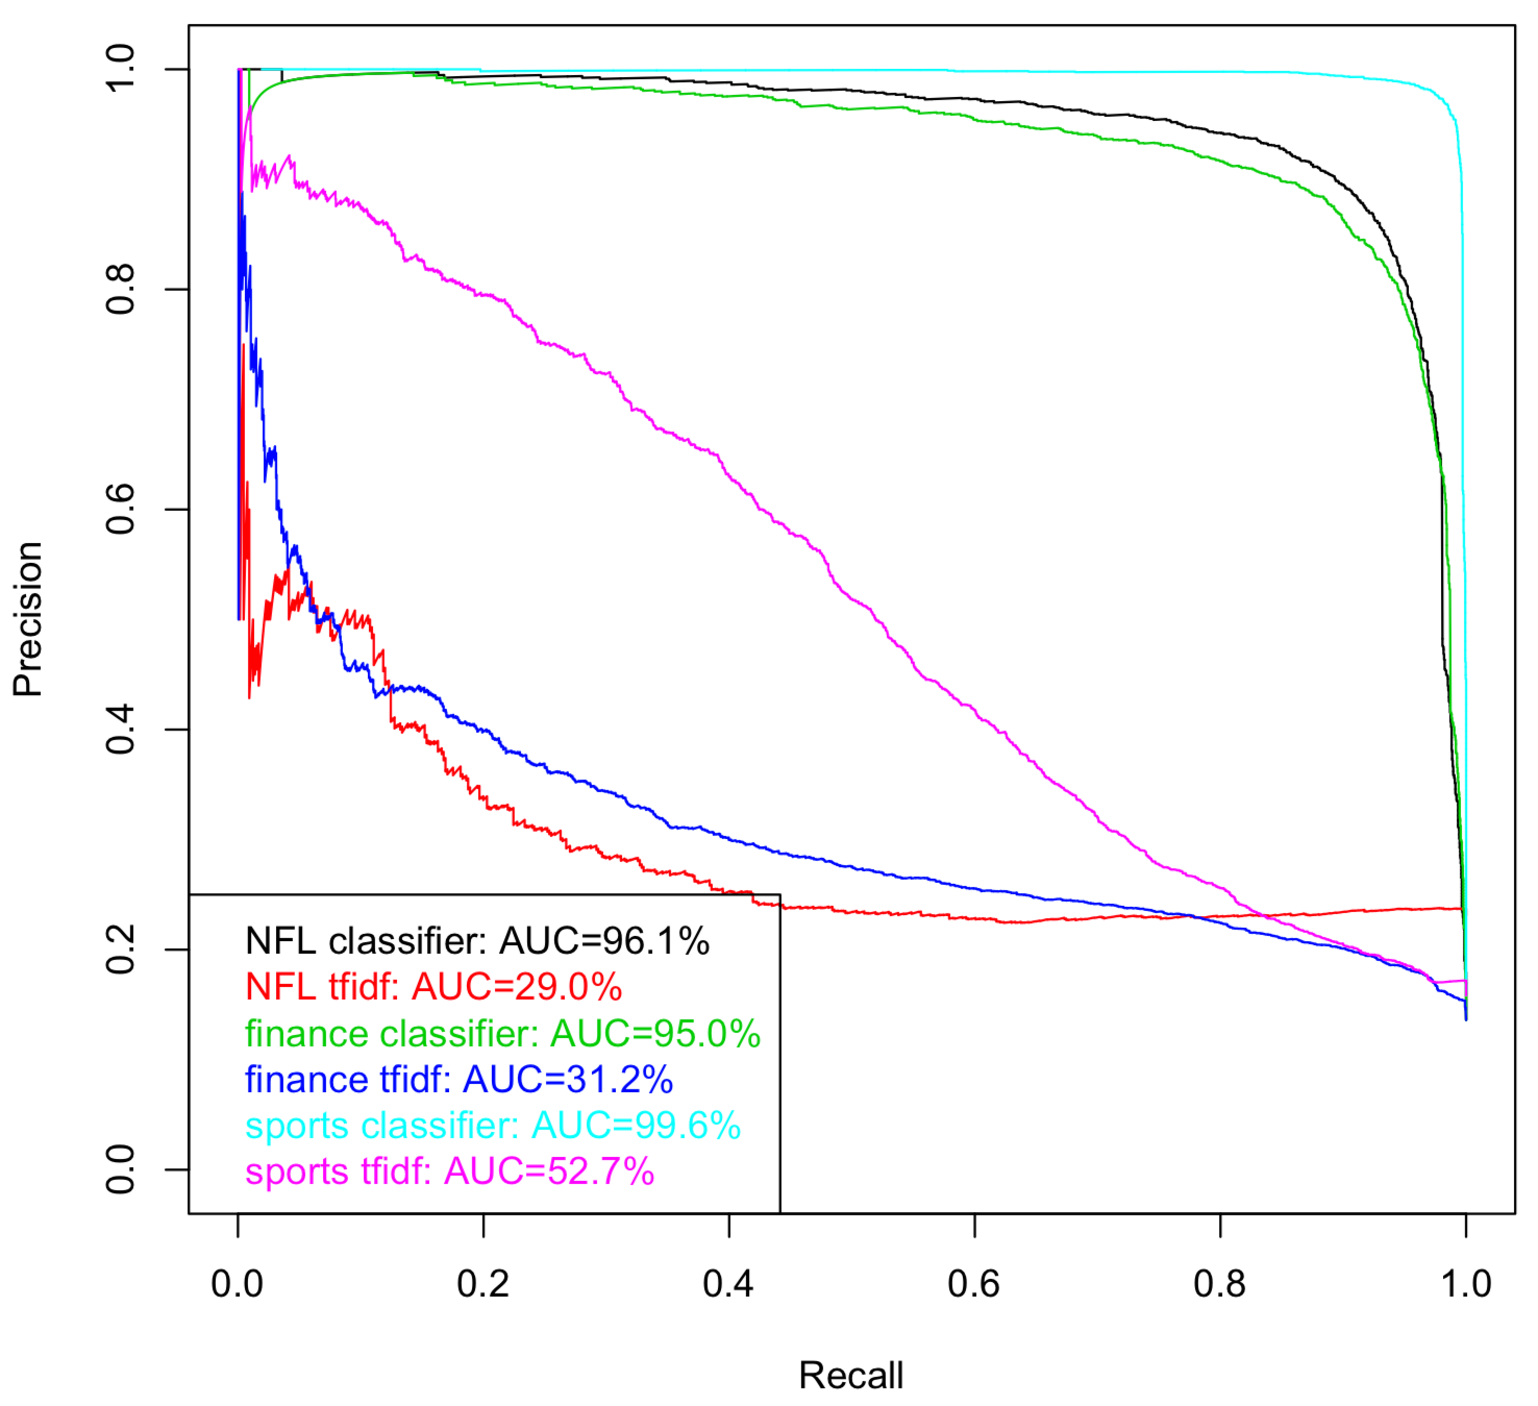
\includegraphics[scale=0.28]{precision-recall6.pdf}

\end{figure*}


\subsubsection{Phase 1}
Here we present the ROC AUC for Sports and Finance under four sets of training 
methodologies (Table~\ref{tag:phase1exp}). The weights for the consolidated 
components (gmp, $\langle \bfu, \bfq \rangle$, etc) are optimized a second 
time with respect to the training set. It is interesting to observe that the 
SRQ with negative regressor pruning results in an ROC curve that dominates all 
other models in both cases. We modified the exponential recency in the 
original dot product model in favor of a completely linear one, to achieve 
optimal ranking performance.


\begin{enumerate}
\item gmp only: $\rm{score} = \alpha \rm{gmp} + \beta \Delta T$;
\item flat dot-product (no SRQ) + gmp (baseline): $\rm{score} = \alpha_0 \rm{gmp} + \alpha_1 \langle \bfu,\bfd\rangle + \beta \Delta T$;
\item SRQ + gmp: $\rm{score} = \alpha_0 \rm{gmp} + \alpha_1 \langle \bfq \circ \bfu, \bfd \rangle + \beta \Delta T$;
\item SRQ with negative pruning + gmp: $\rm{score} = \alpha_0 \rm{gmp} + \alpha_1 \langle \widetilde{\bfq} \circ \bfu, \bfd \rangle + \beta \Delta T$, where $\widetilde{\bfq}_i = 0$ if $\bfq_i \le 0$.
\end{enumerate}

\begin{table}
\caption{Phase 1 multiple models}
\label{tag:phase1exp}
\begin{tabular}{|l|l|l|}
\hline
Method & Sports AUC & Finance AUC\\ \hline
gmp only & 0.58 & 0.62 \\ \hline
flat + gmp & 0.61 & 0.61 \\ \hline
SRQ + gmp & 0.62 & 0.63 \\ \hline
SRQ prune + gmp & 0.64 & 0.65 \\ \hline
\end{tabular}

\end{table}

%\begin{figure}[H]
%\centering
%\caption{Sports ROC} \label{Sports ROC}
%\includegraphics[scale=0.3]{Sports-ROC.pdf}
%
%\end{figure}
%\begin{figure}[H]
%\centering
%\caption{Finance ROC} \label{Finance ROC}
%\includegraphics[scale=0.3]{Finance-ROC.pdf}
%
%\end{figure}


\subsubsection{phase 2}
\input phase2exp

%\subsubsection{Phase 3}
%
%
%
%We illustrate the results in Figure~\ref{DD curve} with a single user session. 
%\begin{figure}[H]
%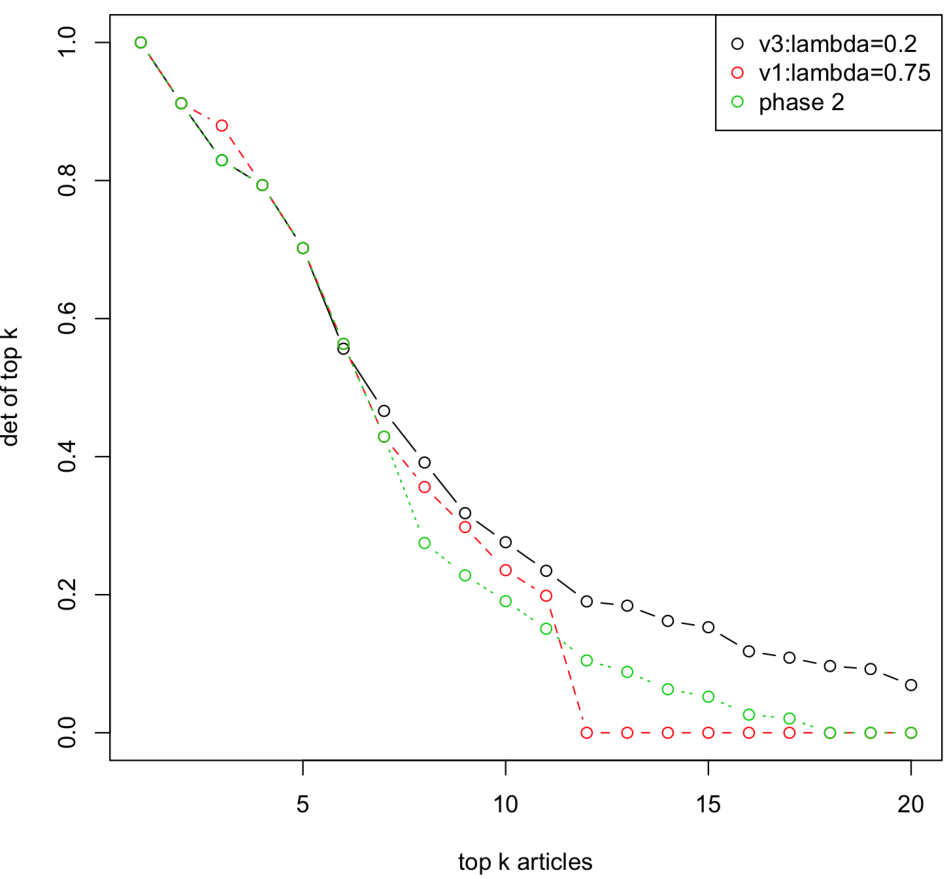
\includegraphics[scale=0.4]{DDcurve.pdf}
%\caption{Determinantal Diversity Curve}\label{DD curve}
%\end{figure}
%
%\begin{figure}[H]
%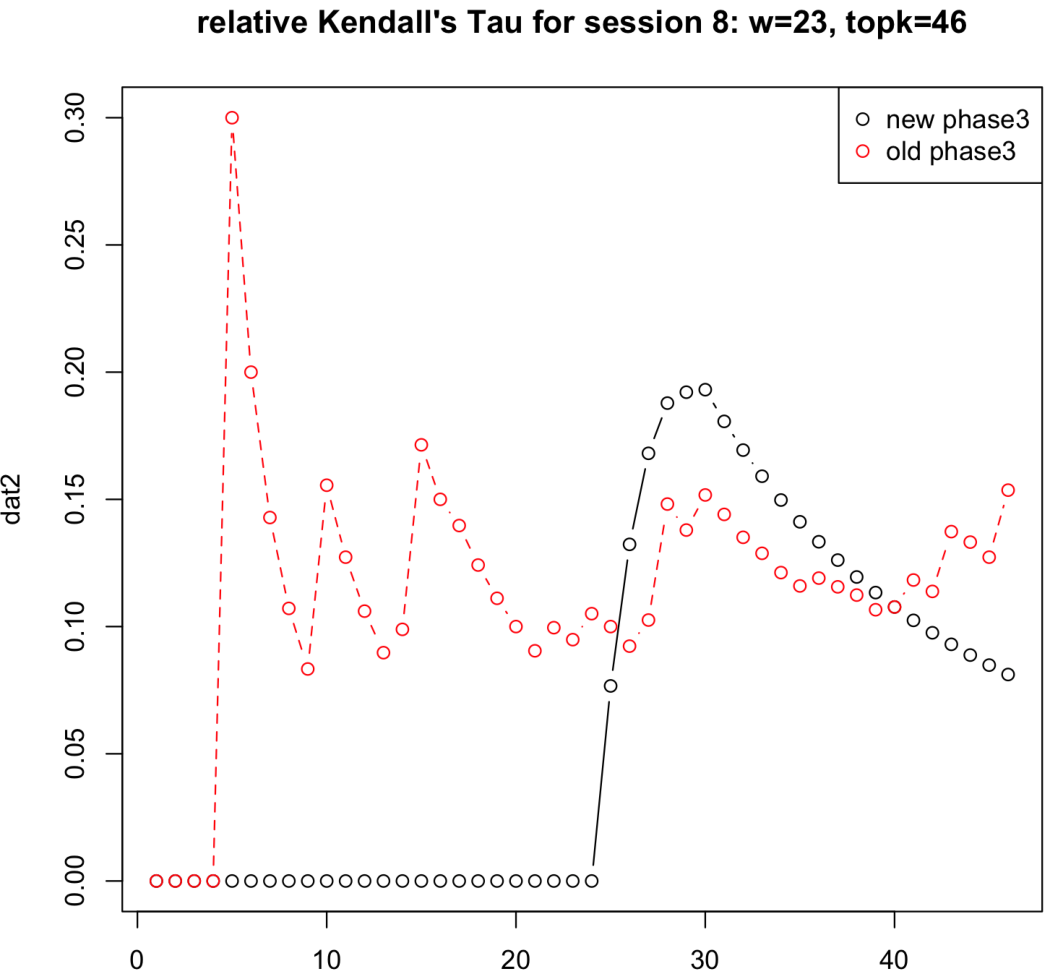
\includegraphics[scale=0.4]{KTcurve.pdf}
%\caption{Kendall's Tau Curve}
%\end{figure}
%
%In terms of determinantal diversity, algorithm v3 outperforms v1 (so-called MMR approach) or with no diversity at all, consistently across all top k positions, with only one exception at position 3. More importantly, by design v3 preserves the original order from phase 2 ranking up to the end of the first window limit, thus the Kendall's metric is flat at 0 for the duration of the first window. After the first window is exceeded, there is a momentary spike in top k Kendall tau metric, followed by rapid decrease to a level below that of v1. 
%
%\appendix
%\section{Diversity Ranking Results} \label{appendix diversity}
%Here we present the top 24 articles ranked by both algorithms v1 and v3 for a randomly chosen session on the Finance stream.
%
%Ranking of finance articles according to algorithm v1:
%\ssmall{
%\begin{verbatim}
%ph2    ph3    headline
%0       0       Carl Icahn says sellers 'completely misinterpreted' Apple's results"
%1       1       Bad Sign for Yahoo: Alibaba's Growth Slows"
%2       2       Steady Fed policy could steady markets"
%4       3       Indonesia Stocks Rise Most in 2 Weeks on Morgan Stanley Upgrade"
%3       4       Electronic Arts Sales Come Up Short in Console Transition"
%11      5       NYSE stocks posting largest volume increases"
%8       6       Ezcorp 1Q results top views, shares jump"
%7       7       VMware Falls 5%: Q1 Rev View In-Line, Year Rev View Beats"
%9       8       AT&T swings to 4th-quarter profit of $6.9 billion on higher revenue"
%14      9       AT&T reports profit on pension gain"
%13      10      Amgen earnings beat forecasts, but 2014 outlook leaves investors cold"
%16      11      AT&T revenue rises in fourth quarter"
%26      12      Check Point Advances to 12-Year High as Earnings Beat Estimates"
%23      13      Seagate Technology Earnings Miss In Difficult Market"
%15      14      Stocks End Higher; Data, Earnings in Focus"
%28      15      Why Swift Transportation (SWFT) Is Rising Today"
%38      16      Dow Today: E.I. Du Pont De Nemours & Company (DD) Lower"
%43      17      Remaking star fund managers to fit inside an ETF"
%29      18      Builders Rise On D.R. Horton Earnings, Home Prices"
%20      19      Stocks Higher In Afternoon; Polaris Trips Sell Rule"
%34      20      Rent-A-Center shares fall on disappointing 4Q"
%52      21      China Credit Repays Principal to Investors of Bailed-Out Trust"
%53      22      Sumitomo Mitsui Quarterly Profit Falls 9.3% on Bond-Trading Drop"
%37      23      Chipotle Earnings Seen Heating Up On Expansion Plans"
%\end{verbatim}}
%
%Ranking of the same 200 articles according to v3 (lambda = 0.10, w=24):
%\ssmall{
%\begin{verbatim}
%ph2    v3    headlines
%0       0       Carl Icahn says sellers 'completely misinterpreted' Apple's results
%1       1       Bad Sign for Yahoo: Alibaba's Growth Slows
%2       2       Steady Fed policy could steady markets
%3       3       Electronic Arts Sales Come Up Short in Console Transition
%4       4       Indonesia Stocks Rise Most in 2 Weeks on Morgan Stanley Upgrade
%7       5       VMware Falls 5%: Q1 Rev View In-Line, Year Rev View Beats
%8       6       Ezcorp 1Q results top views, shares jump
%9       7       AT&T swings to 4th-quarter profit of $6.9 billion on higher revenue
%10      8       NYSE stocks posting largest volume decreases
%13      9       Amgen earnings beat forecasts, but 2014 outlook leaves investors cold
%23      10      Seagate Technology Earnings Miss In Difficult Market
%26      11      Check Point Advances to 12-Year High as Earnings Beat Estimates
%28      12      Why Swift Transportation (SWFT) Is Rising Today
%29      13      Builders Rise On D.R. Horton Earnings, Home Prices
%34      14      Rent-A-Center shares fall on disappointing 4Q
%37      15      Chipotle Earnings Seen Heating Up On Expansion Plans
%38      16      Dow Today: E.I. Du Pont De Nemours & Company (DD) Lower
%41      17      American Airlines posts $2 billion loss on charges
%43      18      Remaking star fund managers to fit inside an ETF
%49      19      Maruti Net Income Misses Estimates After Discounts
%52      20      China Credit Repays Principal to Investors of Bailed-Out Trust
%53      21      Sumitomo Mitsui Quarterly Profit Falls 9.3% on Bond-Trading Drop
%54      22      What to expect from Obamacare bellwether Wellpoint
%61      23      [video] Why hedging will be key this year
%\end{verbatim}}
%
%Version 1 often does not properly eliminate articles with very similar content, judging from their headlines, as  the three almost back-to-back AT\&T articles demonstrate. Equally serious is the observation that many articles under v1 get reversed in their relative order for no apparently good reason. The minimally disruptive nature of v3 makes it an at least locally optimal meta-algorithm on top of phase 2 gbdt ranking.
%
% The following two commands are all you need in the
% initial runs of your .tex file to
% produce the bibliography for the citations in your paper.

\section{Conclusions}
\label{sec:conclusions}
This paper describes a system to recommend contents for multiple semantic 
streams.
%Web portal provides contents for users to browse. 
 We present a semantic stream hierarchy to guide internet users to  browse 
 contents and help them find personally interesting articles more easily and 
 quickly. To solve the content recommendation problem for multiple semantic 
 streams at various depths, we face unique challenges such as scalable 
 multi-layer stream classification and stream ranking. 

% We all know content recommendation is very different from Web search engine.  Search engine provides search results for an issued query, but web portal recommends %content without query. Instead,  users browse the contents. To serve user browse,  In order to solve content recommendation for multiple semantic streams,   not only do we %experience the same challenges as existing work such as recency, and personalization, but we are facing new challenges that 

Several new methods are proposed such as click-based stream classifier and 
using stream-id to improve multiple stream ranking.  All these methods are 
found effective and improved upon baseline model significantly.  

%Our work also presented new results regarding recency handling. Experiments suggest that both relevance and recency were improved, which is a significant progress over the %results of existing work ~\cite{Liu:2010:PNR:1719970.1719976}.  

The whole system is decomposed into three phases: phase 0 deals with 
hierarchical content classification and phase 1 and 2 perform efficient 
ranking. =We demonstrate order of magnitude improvement in precision-recall of 
the 
linear classifier over tfidf approach. Compared with hand-crafted rule-based 
approach, the classifier significantly increases recall while maintaining the 
same or better precision. For phase 1 personalized stream-specific linear 
ranking, we measure the performance in terms of click/skip ROC curves and show 
an increase in Area Under the Curve (AUC) of 3-4\% under model 
\eqref{practical SRQ}  over the stream-independent model. Finally phase 2 
refines the ranking results from phase 1 by taking into account a select set 
of 14 features related to user, document, and their interactions. We observe 
huge CTR and dwell-time gains over the baseline from online user experience 
test.


 In practice, not all 3 phases are applied to all streams uniformly. Some 
 small streams have few articles, or may not need 
 personalization from Phase 1 or Phase 2.  It is flexible to 
 adjust the 3 phases for different steams. This will be examined in an 
 upcoming work.





\bibliographystyle{abbrv}
\bibliography{gs-ranking,ref1,ref3}  % sigproc.bib is the name of the Bibliography in this case






% comments for how to generate the plots in R
\/*
~/Documents/latex/grandslam/plots/

plot(c(0,1),c(0,1),type="n", xlab='Recall', ylab='Precision');

g=file('fin.c=10.predlab');
f=read.table(g);
names(f) = c('pred','label');
library('ROCR');
pred <- prediction(f$pred,f$label);
perf <- performance(pred,'prec','rec');
plot(perf,add=T,col=1);

g=file('fin.tfidf.predlab');
f=read.table(g);
names(f) = c('pred','label');
library('ROCR');
pred <- prediction(f$pred,f$label);
perf <- performance(pred,'prec','rec');
plot(perf,add=T,col=2);

g=file('spt.c=10.predlab');
f=read.table(g);
names(f) = c('pred','label');
library('ROCR');
pred <- prediction(f$pred,f$label);
perf <- performance(pred,'prec','rec');
plot(perf,add=T,col=3);

g=file('spt.tfidf.predlab');
f=read.table(g);
names(f) = c('pred','label');
library('ROCR');
pred <- prediction(f$pred,f$label);
perf <- performance(pred,'prec','rec');
plot(perf,add=T,col=4);

g=file('nflspt.c=10.predlab');
f=read.table(g);
names(f) = c('pred','label');
library('ROCR');
pred <- prediction(f$pred,f$label);
perf <- performance(pred,'prec','rec');
plot(perf,add=T,col=5);

g=file('nflspt.tfidf.predlab');
f=read.table(g);
names(f) = c('pred','label');
library('ROCR');
pred <- prediction(f$pred,f$label);
perf <- performance(pred,'prec','rec');
plot(perf,add=T,col=6);


legend(0,0.25,c('finance classifier: AUC=99.8%','finance tfidf: AUC=31.2%','sports classifier: AUC=99.9%','sports tfidf: AUC=52.7%', 'nfl classifier: AUC=96.3%','nfl tfidf: AUC=29.0%'),text.col=c(1,2,3,4,5,6));

*/

% compute precision recall from a prediction-label space separated file
\/*
#!/bin/bash
# computes pointwise precision recall at 0 threshold
file=$1
pos=`cat $file | awk '{if ($1 > 0) print $0}' | wc -l`
neg=`cat $file | awk '{if ($1 < 0) print $0}' | wc -l`
truepos=`cat $file | awk '{if ($1 > 0 && $2 == 1) print $0}' | wc -l`
trueneg=`cat $file | awk '{if ($1 < 0 && $2 == -1) print $0}' | wc -l`
falsepos=$(( pos - truepos ))
falseneg=$(( neg - trueneg ))
precision=`echo "$truepos / $pos" | bc -l`
recall=`echo "$truepos / ( $truepos + $falseneg )" | bc -l`
echo "precision = " $precision
echo "recall = " $recall
*/



\end{document}
